\documentclass[10pt]{wlpeerj}
\usepackage{mathtools}
\usepackage{soul}

\title{Trafficking synaptic cargo in complex morphologies involves tradeoffs in speed and precision}

\author[1,2,3,*]{Alex H. Williams}
\author[2]{Cian O'Donnell}
\author[4]{Eve Marder}
\author[2,5]{Terrence Sejnowski}
\author[4,*]{Timothy O'Leary}

\affil[1]{Department of Neurosciences, University of California, San Diego, La Jolla, CA 92093, USA}
\affil[2]{Howard Hughes Medical Institute, Salk Institute for Biological Studies, La Jolla, CA 92037, USA}
\affil[3]{Department of Neurobiology, Stanford University, Stanford, CA 94305, USA}
\affil[4]{Volen Center and Biology Department, Brandeis University, Waltham, MA 02454, USA}
\affil[5]{Division of Biological Sciences, University of California at San Diego, La Jolla, CA 92093, USA}
\affil[*]{Address correspondence to: ahwillia@stanford.edu, toleary@brandeis.edu}

\keywords{Synaptic tagging hypothesis, LTP, Transport, Morphology}

\begin{abstract}
Long lived changes in synaptic strength underlie persistent memories and in many cases require activity dependent transcription of plasticity-related genes.
A well-known problem is to understand how appropriate gene products, such as synaptic proteins and mRNAs, get trafficked to the synapses that require them in spite of the complex dendritic arbors and thousands of postsynaptic sites typical of many neurons.
We develop a biophysically-rooted model of microtubule transport, and identify procedures that produce desired distributions of cargo to arbitrarily high precision.
Importantly, these transport systems can be plausibly encoded by simple, localized biochemical reactions.
The model predicts that the precise and flexible delivery of synaptic cargo requires the capture of synaptic cargo to occur on a slower timescale than the movement of cargo across the microtubule network.
Thus, neurons must find a compromise between the specificity and speed with which synaptic materials are delivered and long-lived connectivity patterns are formed.
\end{abstract}

% OLD ABSTRACT:
%Long lived changes in synaptic strength underlie persistent memories and in many cases require activity dependent transcription of plasticity-related genes.
%A well-known problem is to understand how appropriate gene products, such as synaptic proteins and mRNAs, get trafficked to the synapses that require them in spite of the complex dendritic arbors and thousands of postsynaptic sites typical of many kinds of neuron.
%Using a simple, biophysically-rooted model of microtubule transport we show that rapid delivery of plasticity-related cargo entails loss of specificity in the synapses that eventually receive it.
%The model predicts that neurons must balance the biochemical parameters that control trafficking to find a compromise between the precision and speed with which long-lived connectivity patterns are formed.
%Conversely, imbalances in transport parameters could lead to hypo-, or hyperconnectivity as well as loss of precision in associative memory, identifying a potential role for transport machinery in brain disorders that exhibit connectivity and plasticity phenotypes.


\begin{document}

\flushbottom
\maketitle
\thispagestyle{empty}

\section*{Introduction}

Neurons often have complex dendritic trees, reflecting the dense and structured synaptic connectivity that supports nervous system function.
In order to maintain appropriate connectivity, or to alter it as a means of encoding memories, numerous enzymes and macromolecules need to be transported along dendrites to the synapses that need them.
How is this logistical problem solved at the subcellular level? And how might a biologically plausible solution constrain the behavior of synaptic plasticity `rules' and learning in general?

Transport along dendrites is mediated by motor proteins (kinesins and dyneins) that walk along microtubules, carrying cargo at a rate that far exceeds passive diffusion [REFS].
The mechanisms that detach and sequester cargo at specific places in dendrites are not fully understood, but are known to depend on local biochemical signals that can be influenced by synaptic activity, such as transient elevations in cyclic AMP or $[Ca^{2+}]$ \cite{Mironov_2007,Wang_2009}.
It is therefore conceivable that synaptic cargo transport is controlled in a distributed fashion, in which synapses that require cargo trigger its release from the motor protein complexes as they pass.
This idea is a variant of the well-known synaptic tagging hypothesis \citep{Frey_1997}, which proposes that synapses produce a biochemical `tag' that signals a requirement for synaptic building blocks as part of the plasticity process.

Not all aspects of synaptic plasticity require delivery of cargo from the soma. For example, some forms of long-term potentiation (LTP) depend on local protein synthesis and can function in isolated dendrites [REFS].
However, in the long run, the mRNAs and the machinery that supports such plasticity needs to be replenished. Moreover, many long-lasting forms of synaptic plasticity rely on anterograde transport of mRNAs \citep{Kandel_2001,Puthanveettil_2008} and specific mRNAs are known to be selectively transported to regions of heightened synaptic activity \citep{Steward_1998,Steward_2001,Moga_2004} or to developing synaptic contacts \citep{Lyles_2006}.
The interplay between global distribution and local plasticity mechanisms therefore demands attention.

From simple assumptions about the dynamics of active dendritic transport we develop a model that can account for activity-dependent accumulation of molecular cargo at synaptic sites in realistic neuronal morphologies.
Within this framework, we identify several ways in which local biochemical mechanisms can be orchestrated to produce arbitrarily complex distributions of molecular cargo.
In addition to addressing the logistical challenges of dendritic transport, we identify several constraints the precision, flexibility, and speed of cargo delivery inherent to this model.

\hl{}

\section*{Results}

\subsection*{Model description}

\begin{figure}[!tb]
\begin{center}
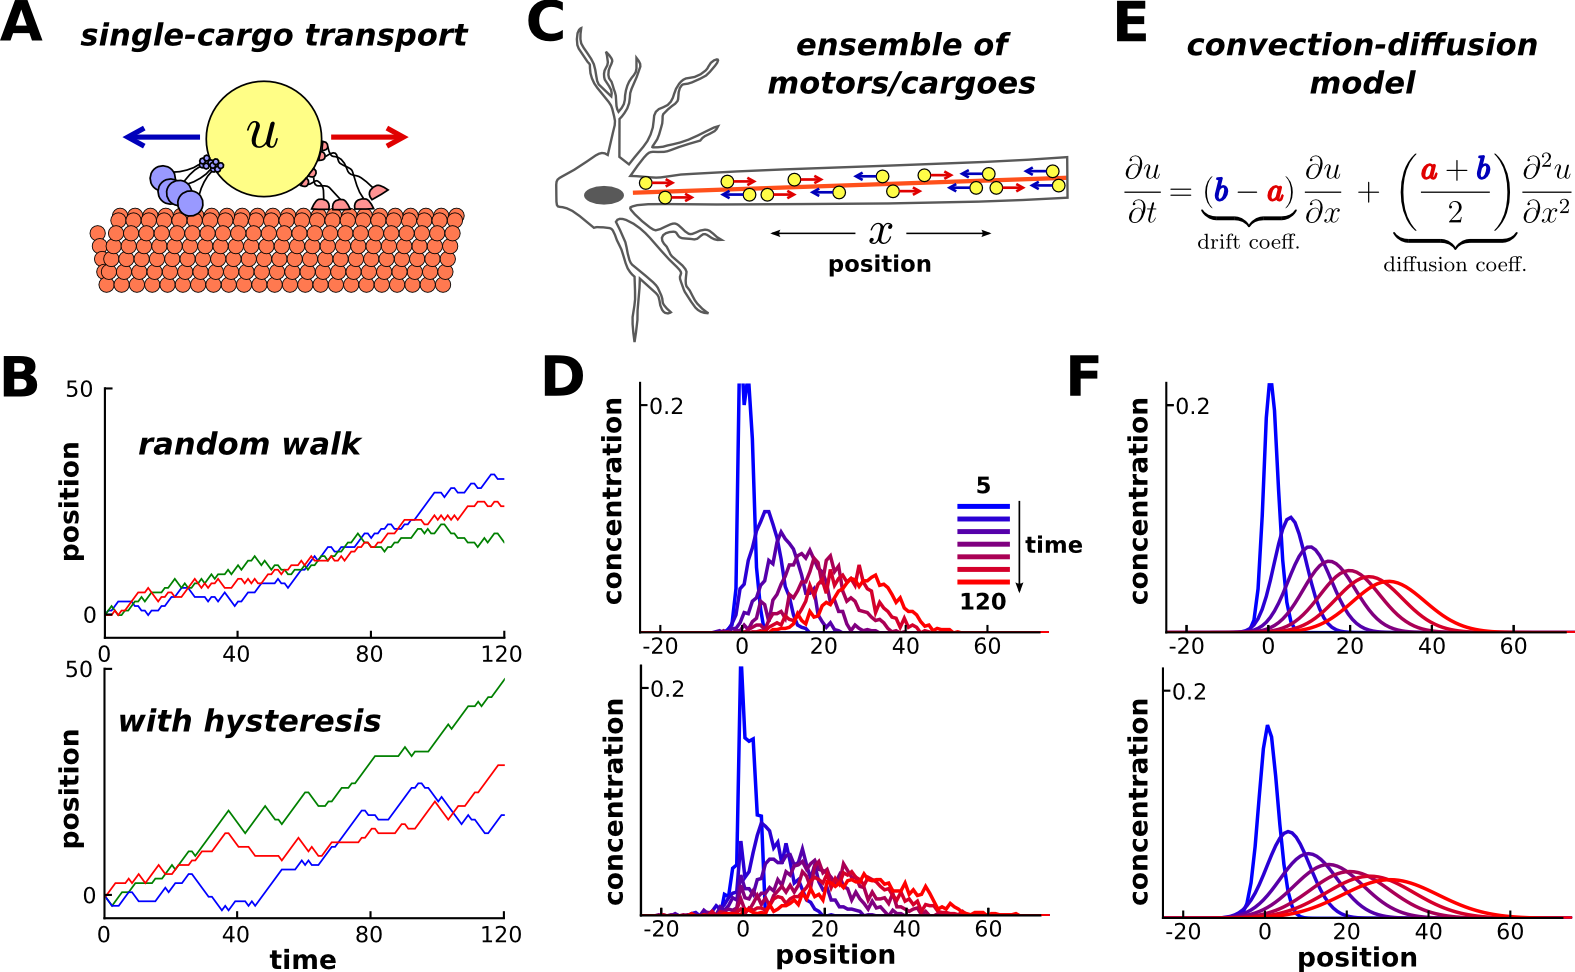
\includegraphics[width=0.9\columnwidth]{00_stochastic.png}
\caption{Model of microtubular transport.
\textbf{(A)} Synaptic cargo, $u$, undergoes stochastic back-and-forth movements driven by opposing motor proteins.
\textbf{(B)} Three example random walks on a cable representing the movement of individual cargoes. In a simple random walk, each movement is independent of previous movements (top panel); longer run lengths result from adding history-dependence to the model, such that each movement is likely to continue in the same direction as the previous step (bottom panel).
\textbf{(C)} An ensemble of synaptic cargoes transported along the length of a neurite.
\textbf{(D)} The concentration profile of transported cargo along a cable over time, simulated as 1,000 independent random walks. Simulations with (bottom) and without (top) history-dependence.
\textbf{(E)} In the limit of many individual particles, the concentration of $u$ is modeled by the convection-diffusion partial differential equation. The parameters, $a$ and $b$, respectively scale the anterograde and retrograde rate of transport (see equation 1).
\textbf{(F)} The convection-diffusion model provides a good fit for the simulations in panel D.
}
\end{center}
\end{figure}

Transport along microtubules is mediated by kinesin and dynein motors, which mediate anterograde and retrograde transport, respectively \citep{Hirokawa_2010,Gagnon_2011}.
Cargo is often simultaneously bound to both forms of motor protein, resulting in stochastic back-and-forth movements with a net direction determined by the balance of opposing movements \citep{Hancock_2014,Buxbaum_2014b} (Fig. 1A).

To obtain a general model that can accommodate variations in the biophysical details, we consider microtubule-based transport as a biased random walk along a one-dimensional cable \citep{Bressloff_2006,Newby_2010,Bressloff_2009}.
For each time step, the cargo moves left, right, or remains in the same place.
In the simplest model, the probabilities associated with each movement are fixed and independent across each time step (Fig. 1B, top panel).
A potentially more realistic model incorporates \textit{hysteresis} into the biased walk (see Methods). In this case, the cargo is more likely to continue in the same direction as it moved on the previous time step (Fig. 1B, bottom panel; see, e.g., \cite{Soundararajan_2014}).

While the position of individual cargoes can be highly stochastic, the net movement of a population of cargoes (Fig. 1C) is predictable.
Figure 1D shows the distribution of 1000 molecules over time with (top panel) and without (bottom panel) hysteresis.
In both cases, these simulations can be well-fit by an convection-diffusion partial differential equation (Fig. 1E-F), which is easier to analyze because it is deterministic and contains fewer variables \citep{Smith_2001}.

The convection-diffusion equation can be numerically simulated by discretizing a dendritic tree into small compartments, and considering the movement of cargo between neighboring compartments as a chemical reaction with first order kinetics. In an unbranched cable with $N$ compartments, the mass-action model is:
\begin{equation}
u_1 \xrightleftharpoons[b_1]{a_1} u_2 \xrightleftharpoons[b_2]{a_2} u_3 \xrightleftharpoons[b_3]{a_3} ~...~ \xrightleftharpoons[b_{N-1}]{a_{N-1}} u_N
\end{equation}
where $u_i$ is the amount of cargo in each compartment, and $a_i$ and $b_i$ respectively denote local rate constants for anterograde and retrograde transport; these parameters determine the local diffusion and drift coefficients as shown in figure 1E (see Methods). Similar mass-action schemes can be constructed to model transport in branched morphologies (Fig. 2A).

\hl{MOVE THIS PARAGRAPH TO METHODS/DISCUSSION?} A central assumption of this model is that the movement of molecules between neighboring compartments is a stochastic and memoryless process. This assumption is reasonable if the \hl{run length (jargon?)} of molecular motors is comparable to the size of the compartments; this appears to be the case under many \citep{Muller_2008,Verbrugge_2009}, thought not necessarily all \citep{Dynes_2007} circumstances (see Discussion). In simulations, we observed that this model was not very sensitive to violations of this assumption; the population dynamics of cargoes with substantial run lengths could still be well-fit by this class of models (Fig. 1F, lower panel; Supplementary Fig?).

\subsection*{A simple rule achieves desired spatial distributions of cargo}

The exchange of $u$ between neighboring compartments approaches an equilibrium/steady-state ($ss$) distribution over time. In an unbranched cable, this occurs precisely when:
\begin{equation}
\frac{u_i}{u_{i+1}} \Bigg|_{ss} = \frac{b_i}{a_i}
\end{equation}
(see Methods). Thus, the local trafficking rates, $a_i$ and $b_i$, can be tuned to produce a desired spatial distribution of cargo. Let $\tilde{u}$ denote the desired steady-state level of $u$ in each compartment. For example, $\tilde{u}_i$ might refer to the local concentration of biochemical signal that ``tags'' synapses for plasticity \citep{Frey_1997}; such a tag might be positively correlated to the desired level of delivered cargo. To match this desired distribution, the ratio of local trafficking rates should satisfy:
\begin{equation}
\frac{b_i}{a_i} = \frac{\tilde{u}_i}{\tilde{u}_{i+1}}
\end{equation}

\begin{figure}[!tb]
\begin{center}
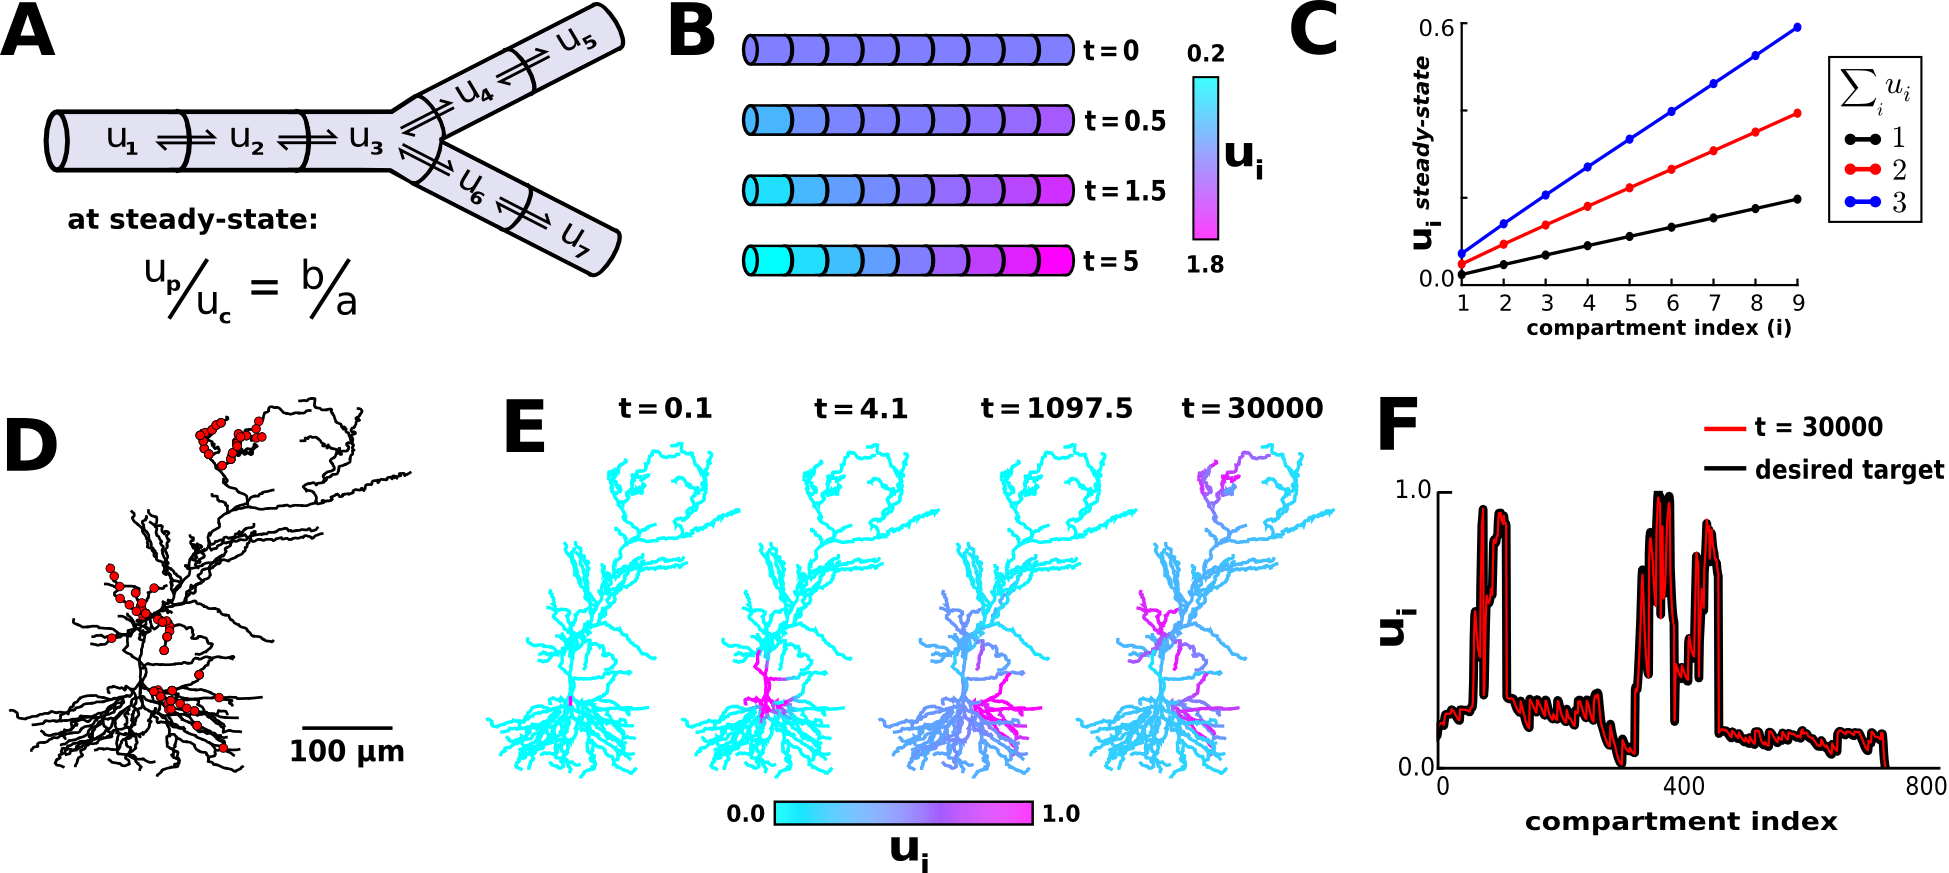
\includegraphics[width=0.9\columnwidth]{01_mass_action.png}
\caption{Local trafficking parameters determine the spatial distribution of biomolecules by a simple rule.
\textbf{(A)} Diagram of the mass action transport model for a simple branched morphology.
%The steady-state ratio of $u$ between any two neighboring compartments is equal to the reciprocal ratio of the trafficking rate constants between those compartments.
\textbf{(B)} A simulation of a nine compartment cable, with trafficking rate constants set to produce a linear gradient using the steady-state relation shown in panel A.
%The initial distribution of $u$ is uniform (t=0); over time the system achieves the desired linear gradient (steady-state occurs around t=5, in this example).
\textbf{(C)} The slope of the linear gradient shown in panel B is determined by the total amount of $u$ present in the model; the slope increases as more of $u$ is present, but the linear profile is preserved.
\textbf{(D)} A model of a CA1 pyramidal cell with 742 compartments based on \cite{Migliore_2012}; excitatory synapses were added at the locations marked by red dots. 
\textbf{(E)} The average membrane potential in each compartment of the CA1 model cell was used to define a desired spatial distribution, and transport rate constants were chosen according to equation (4). The desired spatial distribution of cargo emerges over time, after starting in the soma.
\textbf{(F)} The desired and steady-state profile of $u$ for each compartment in the simulation shown in panel E.
}
\end{center}
\end{figure}

For example, a linear expression pattern emerges when $\tilde{u}_i \propto i$, resulting in $b_i / a_i = i / i + 1$ (Fig. 2B).
This rule produces the expected linear expression gradient with the slope controlled by tuning the total amount of cargo in the cable (Fig. 2C).

These results extend directly to branched morphologies (see Methods). For any pair of connected compartments:
\begin{equation}
%\frac{u_p}{u_c} \Bigg|_{ss} = \frac{b}{a}
\frac{b}{a} = \frac{\tilde{u}_p}{\tilde{u}_c}
\end{equation}
where $u_p$ is the level in the ``parent" compartment (closer to soma) and $u_c$ is the level in the ``child" compartment (closer to periphery); $b$ and $a$ refer to the local transport rate constants between this pair of compartments.


\hl{MOVE THIS PARAGRAPH TO DISCUSSION OR DELETE?} These rules could be locally implemented by simple biochemical reaction networks. Consider the cytoplasmic calcium concentration, $[ca]_i$, as a candidate second messenger. Increases in $[ca]_i$ simultaneously arrest anterograde and retrograde microtubular transport \citep{Wang_2009}. That is, for any pair of compartments, the anterograde rate constant is determined by calcium in the parent compartment, $a = f([ca]_p)$,  and the retrograde rate constant is determined by calcium in the child compartment, $b = f([ca]_c)$, where $f$ is a function that describes how calcium alters the transport rates. This results in:
\begin{equation}
\frac{b}{a} = \frac{f([ca]_c)}{f([ca]_p)} = \frac{\tilde{u}_p}{\tilde{u}_c}
\end{equation}
where $\tilde{u}_i = 1/f([ca]_i)$.


To test the plausibility of this model in a complex morphology, we extended an existing multi-compartment model of a CA1 pyramidal neuron \citep{Migliore_2012}. Excitatory synaptic input was delivered to 120 locations within three dendritic regions (red dots, Fig. 2D), and the average membrane potential in each electrical compartment determined the target level $\tilde{u}_i$ in each compartment (Methods). This models how molecular cargo could be selectively trafficked to active synaptic sites. Figures 2E and 2F confirm that the spatial distribution of $u$ approaches the desired steady-state.

\subsection*{Convergence rate}

Biochemical processes are time-sensitive.
For example, newly synthesized proteins must be delivered to synapses within $\sim$1 hour to support long-term potentiation in CA1 pyramidal cells \citep{Frey_1997,Frey_1998}.
It is therefore of substantial interest to examine factors that influence the speed of transport in the model.

In equations (4) and (5), we implicitly required each $\tilde{u}_i > 0$ in order to avoid division by zero.
Intuitively, if $\tilde{u}_i = 0$ for some compartment, then no cargo can flow through that compartment, cutting of more peripheral compartments from the transport system.
Similarly, if certain $\tilde{u}_i$ are nearly equal to zero, then transport through these compartments will act as a bottleneck for transport, and convergence to the desired distribution will be slow.

Figure 3 illustrates and analyzes this intuition in a simple three compartment model.
The two compartments on the end of the cable have the same desired level, $\tilde{u}_1 = \tilde{u}_3$; the middle compartment acts as a bottleneck when $\tilde{u}_2$ is very small (Fig. 3A).
This results in the mass-action model:
\begin{equation}
u_1 \underset{x}{\overset{\epsilon}{\rightleftharpoons}} u_2 \underset{\epsilon}{\overset{x}{\rightleftharpoons}} u_3
\end{equation}
We assume that $u$ begins at one end of the cable, and examine the how taking $\epsilon$ to zero affects the convergence rate.
Figure 3B shows that the convergence rate slows dramatically as $\epsilon$ decreases.
This can be can be analyzed using basic linear systems theory; the convergence rate is given by the non-zero eigenvalue with smallest magnitude, which can be thought of as a rate-limiting step or process for the system (Methods, Supp. Fig. 1).
Simulations confirmed this analysis and showed that the convergence rate diverges to infinity as $\epsilon$ approaches zero (Fig. 3C).

\begin{figure}[!tb]
\begin{center}
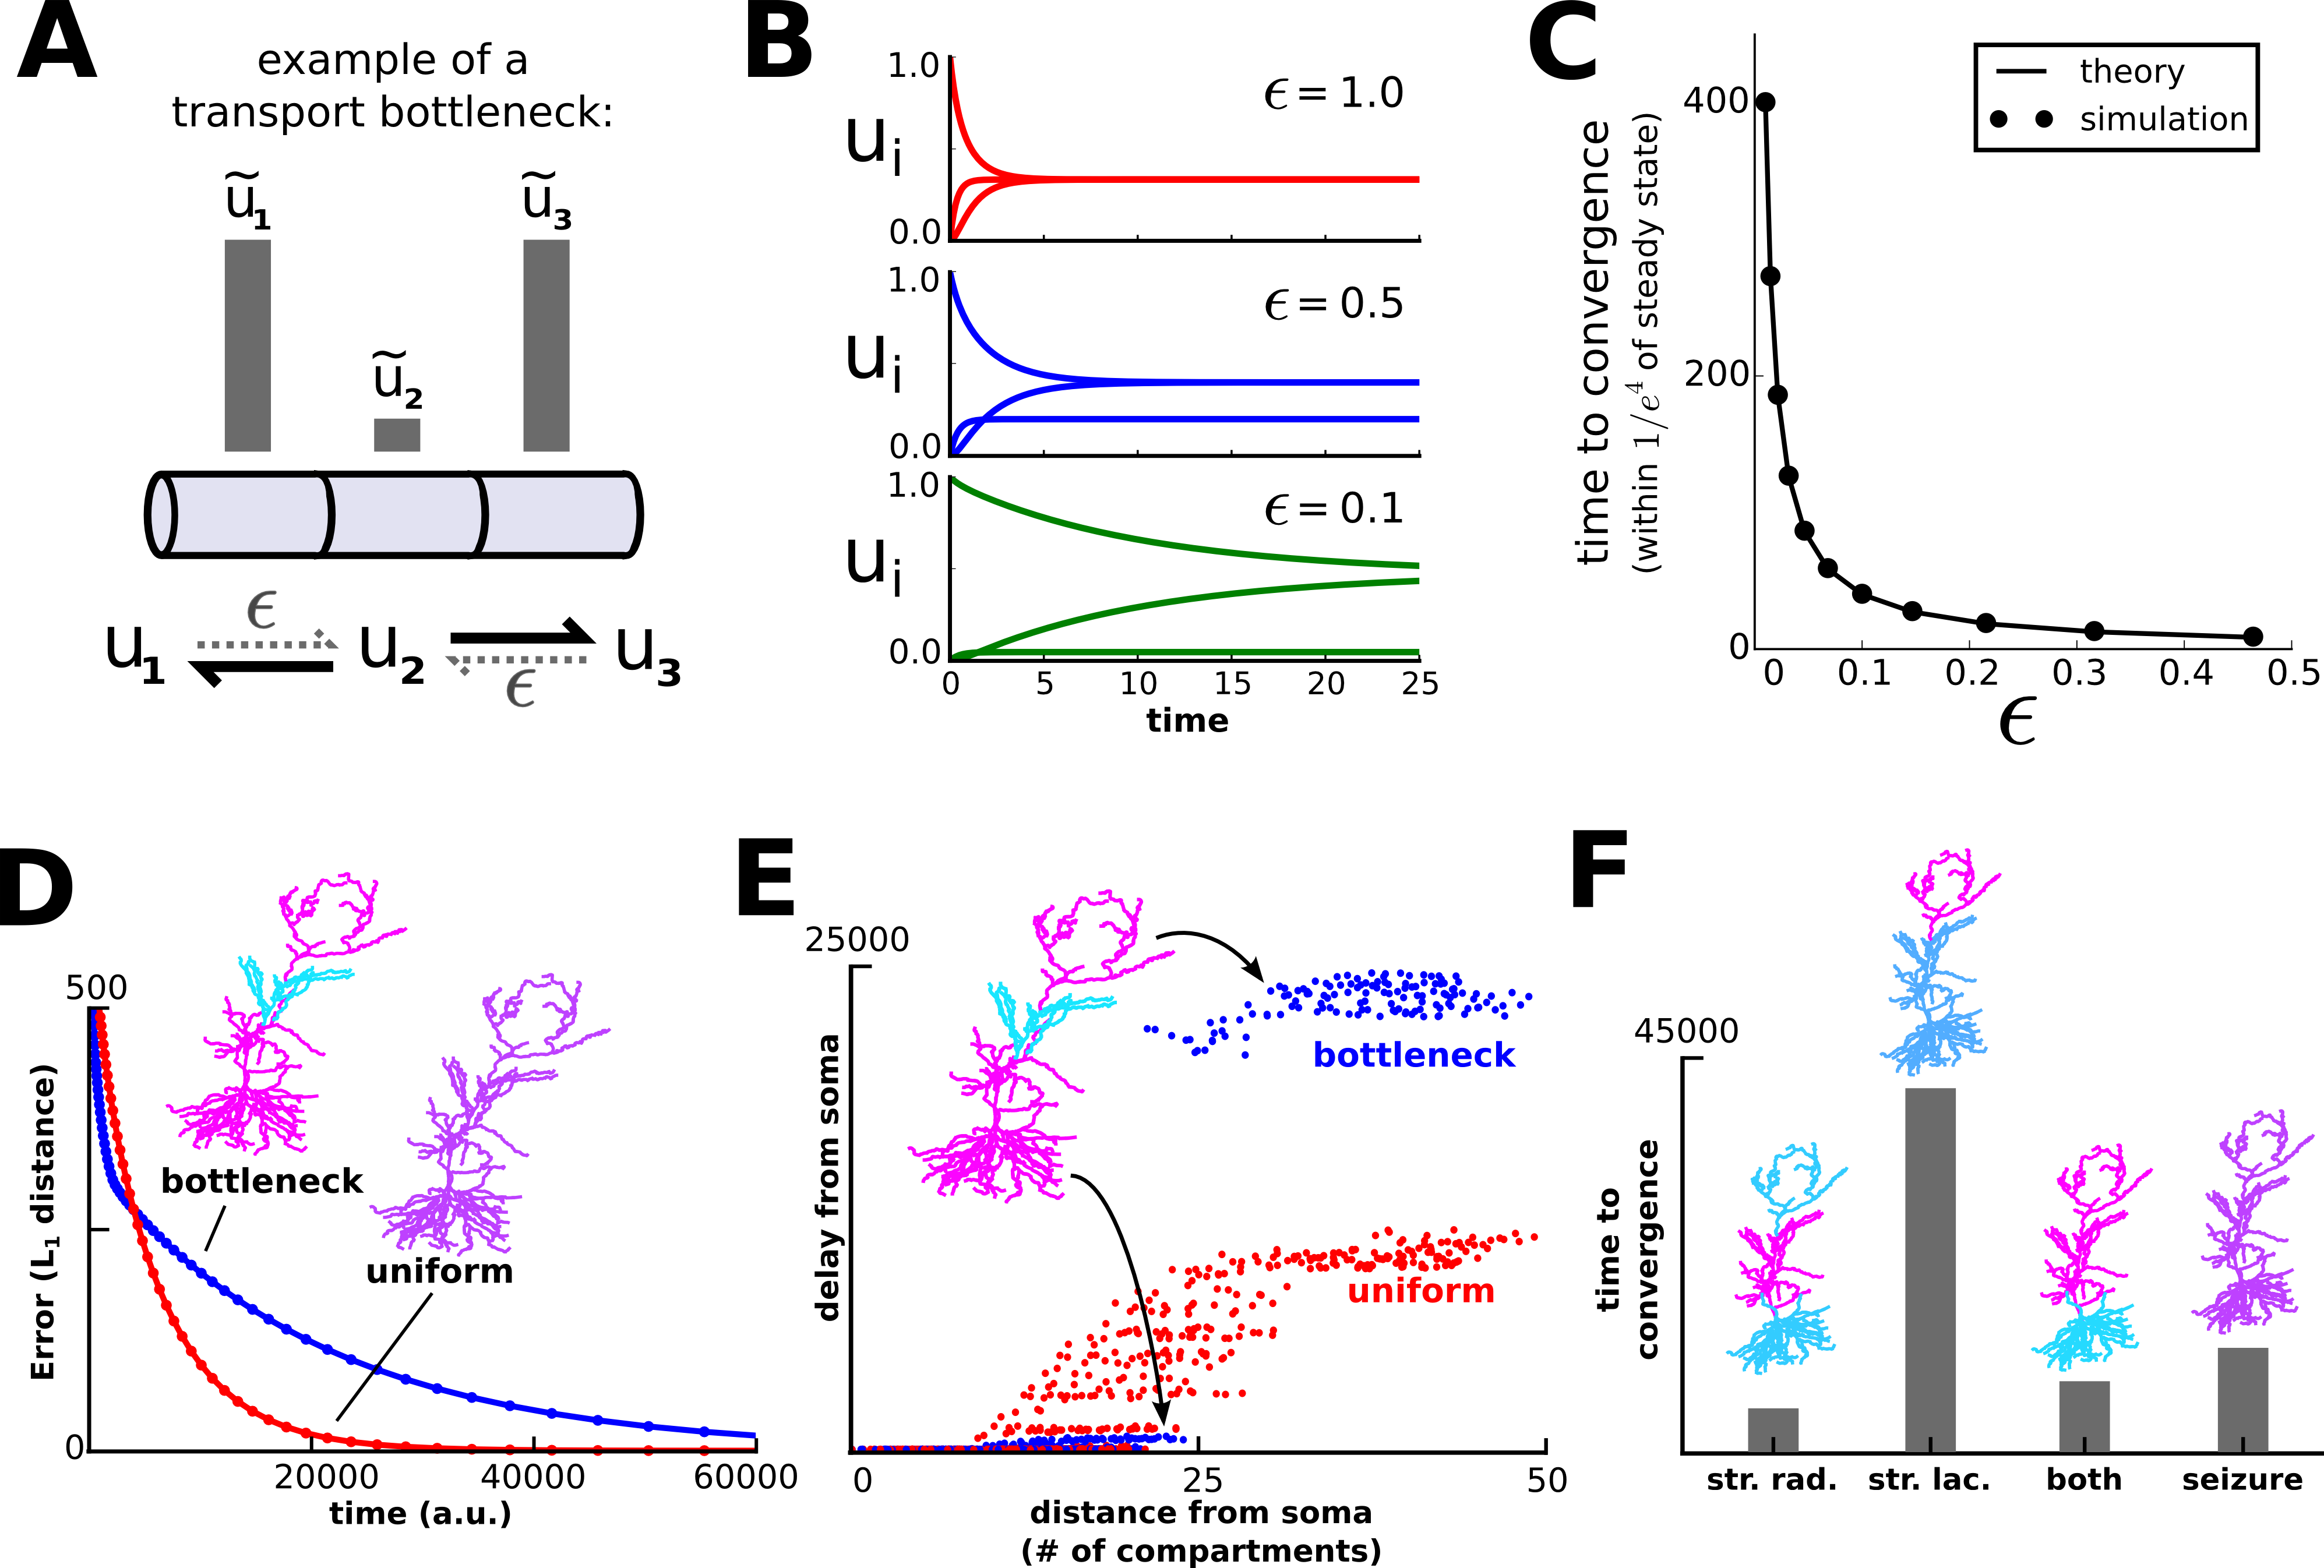
\includegraphics[width=0.9\columnwidth]{03_convergence.png}
\caption{ Convergence to steady-state is slow when molecules must be transported across bottlenecks ---compartments with low target levels.
\textbf{(A)} A three-compartment transport model, with the middle compartment acting as a bottleneck. The vertical bars represent the desired steady-state level of $u$ in each compartment. The rate of transport into the middle compartment is small ($\epsilon$, dashed harpoons) relative to transport out of the middle compartment.
\textbf{(B)} As $\epsilon$ decreases, the model converges more slowly and the steady-state level decreases in the middle compartment.
\textbf{(C)} Simulations (black dots) confirm that the time to convergence is given by the smallest non-zero eigenvalue of the system (analytically calculated line). This eigenvalue can be thought of as the rate-limiting step of the system.
\textbf{(D)} Convergence ($L_1$ distance) to a uniform target distribution (red line) is faster than a target distribution containing a bottleneck (blue line) in the CA1 model.
\textbf{(E)} For all compartments that reach a threshold level ($u_i = 0.001$), the simulated time it takes to reach threshold is plotted against the distance of that compartment to the soma.
\textbf{(F)} Predicted convergence times for various target distributions (str. rad., stratum radiatum; str. lac., stratum lacunosum/moleculare).}
\end{center}
\end{figure}

Qualitatively similar results were obtained in the multi-compartment CA1 neuron model.
The model converged to a uniform target distribution more quickly than to a ``bottleneck" target distribution, in which the middle third of the apical dendrite had low steady-state levels of cargo (Fig. 3D).
Each pair of anterograde and retrograde rate constants were normalized to sum to one; thus, differences in convergence were not due to the scale of the trafficking rate constants.

In addition to this global view of convergence (Fig. 3D), we considered how the transport bottleneck affected transport to individual dendritic compartments.
Consider a scenario where transported cargo produces a local chemical reaction after a critical concentration threshold is reached; for example, a recently potentiated synapse might be stabilized after enough plasticity-related factors are delivered from the soma.
Figure 3E plots the transport delay, or duration of time it took for $u_i$ to reach a pre-defined threshold for each compartment.
We observed qualitatively similar results for different threshold values (data not shown).

As expected, introducing a bottleneck caused much longer delays to compartments distal to that bottleneck (Fig. 3E, upper right portion of plot).
Interestingly, the presence of a bottleneck also \textit{shortens} the transport delay to proximal compartments, compared to the uniform target distribution (Fig. 3E, lower left portion of plot).
This occurs because cargo delayed by the bottleneck spreads throughout the proximal compartments, reaching higher levels earlier in the simulation.

One experimentally testable prediction of this analysis is that transport to distal compartments should be quickened by allowing higher levels of $u$ into the proximal compartments at steady-state (Fig. 3E).
This might be tested by characterizing the convergence time of a retrogradely transported molecule that aggregates at recently activated synapses, such as \textit{Arc} mRNA (\citet{Steward_1998}, see discussion).
To illustrate this in the model CA1 cell, we characterized the time course of transport to the distal apical dendrite (stimulating stratum lacunosum/moleculare), proximal apical dendrite (stimulating stratum radiatum), entire apical dendrite (stimulating both layers), and entire cell (seizure). Interestingly, the model converged more slowly to distal input alone, than to paired distal and proximal input, or to an entirely uniform distribution (Fig. 3F).

\subsection*{Microtubular trafficking, detachment and degradation on separated time scales}

The models above present a simple hypothesis for controlling molecular transport along an intricate system of microtubules.
While certain types of molecular cargo stay on the microtubule network (e.g. mitocondria), others detach from the microtubules after a reaching a desired location.
For example, dendritic mRNAs are transported within densely-packed granules, and can be locally released following granule disassembly \citep{Krichevsky_2001,Buxbaum_2014a}.
We model the detachment from the microtubule network as an irreversible process, and include a compartment-specific degradation reaction. This results in the following mass-action model:
\begin{equation}
\begin{array}{cccccccc}
u_1 & \overset{a_1}{\underset{b_1}{\rightleftharpoons}} &
u_2 & \overset{a_2}{\underset{b_2}{\rightleftharpoons}} &
u_3 & \overset{a_3}{\underset{b_3}{\rightleftharpoons}} &
u_4 & \overset{a_4}{\underset{b_4}{\rightleftharpoons}} ...
\\
c_1 \Bigg\downarrow \phantom{c_1} & &
c_2 \Bigg\downarrow \phantom{c_2} & &
c_3 \Bigg\downarrow \phantom{c_3} & &
c_4 \Bigg\downarrow \phantom{c_4} & 
\\
u_1^\star &  &
u_2^\star &  &
u_3^\star &  &
u_4^\star &   
\\
d_1 \Bigg\downarrow \phantom{d_1} & &
d_2 \Bigg\downarrow \phantom{d_2} & &
d_3 \Bigg\downarrow \phantom{d_3} & &
d_4 \Bigg\downarrow \phantom{d_4} & 
\\
\varnothing &  &
\varnothing &  &
\varnothing &  &
\varnothing &  
\end{array}
\end{equation}
As before, a molecule $u$ is transported along a network of microtubules (top row, in equation 6).
In each compartment, molecules can irreversibly detach from the microtubules in a reaction $u_i \xrightarrow{c_i} u_i^\star$, where $u^\star$ denotes the biochemically active form of $u$, which is assumed to be inactive during transport.
The final reaction, $u_i^\star \xrightarrow{d_i} \varnothing$, models degradation in each compartment.
Note that only $u^\star$ is subject to degradation; the molecule is assumed to be protected from degradation during transport.
This model can be extended to branched morphologies (Fig. 3A).

\begin{figure}[!tb]
\begin{center}
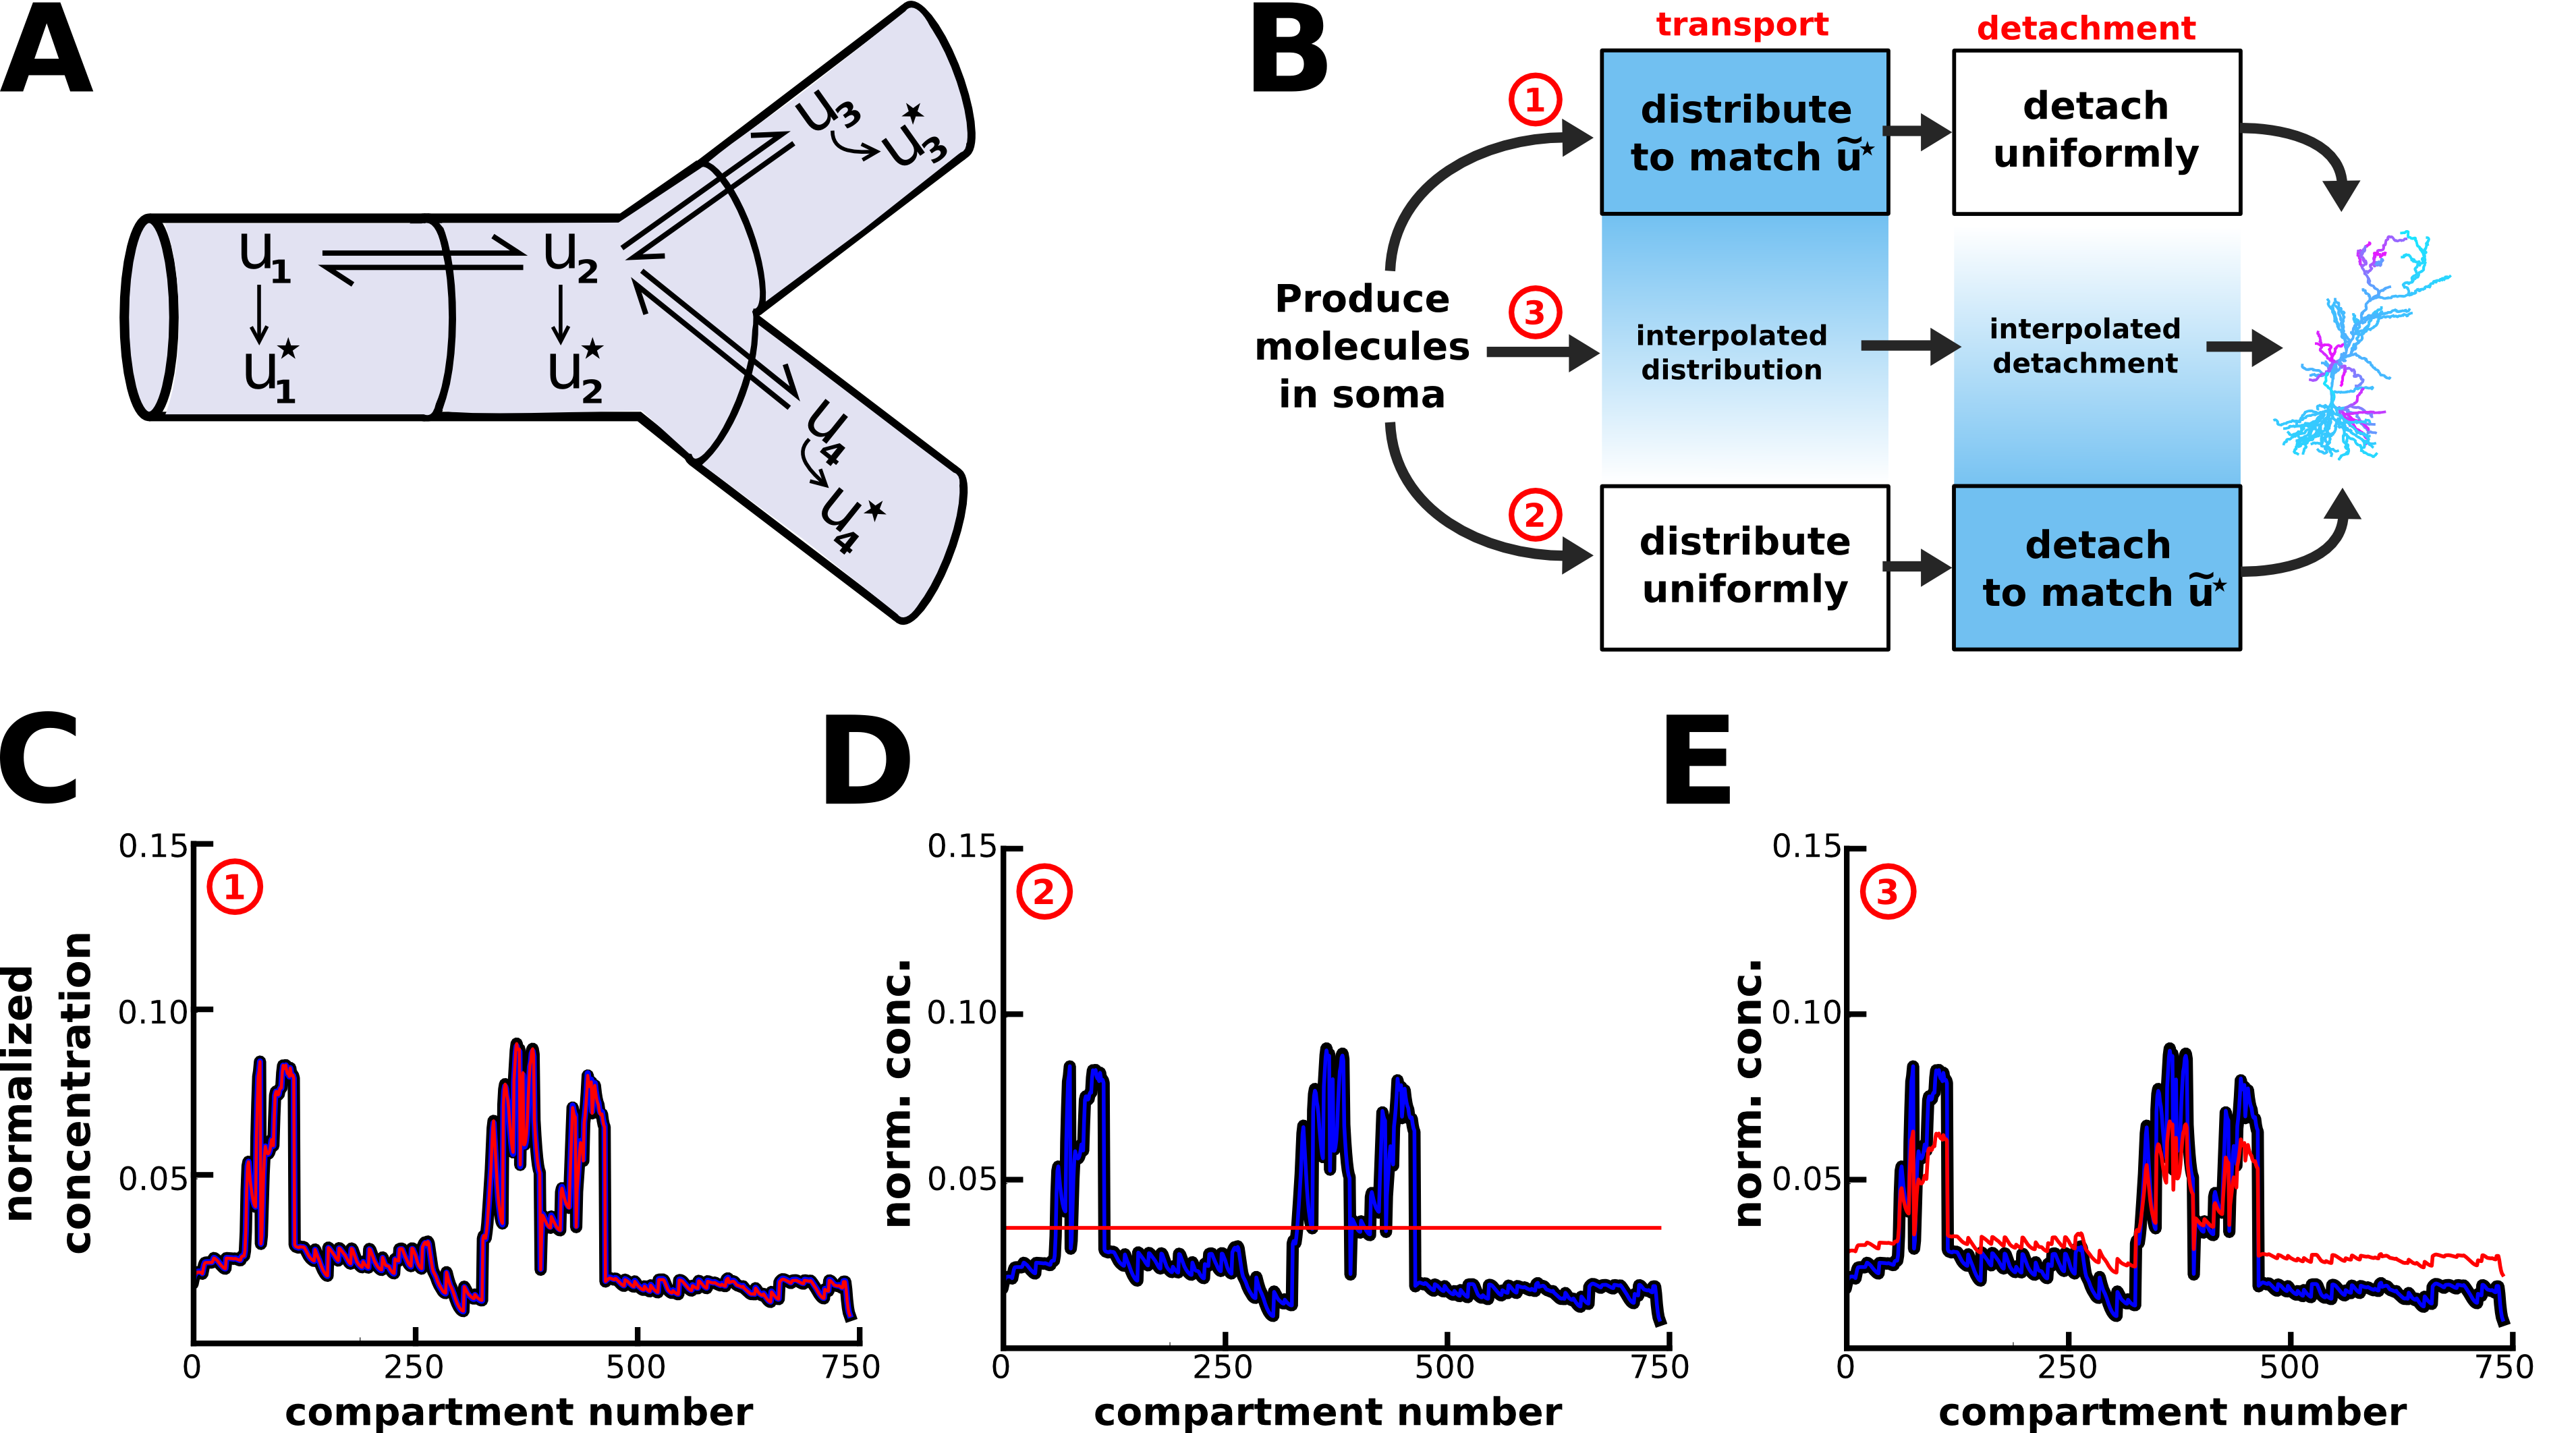
\includegraphics[width=0.9\columnwidth]{04_sushi_belt.png}
\caption{Multiple strategies for transport in a model including nonuniform microtubular detachment/activation.
\textbf{(A)} Schematic of microtubular transport model with irreversible detachment in a branched morphology. The localized degradation reactions ($u^{\star}_i \xrightarrow{d_i} \varnothing$) is omitted.
\textbf{(B)} Multiple strategies for producing a desired distribution of activated biomolecules ($\tilde{u}^{\star}$). When the timescale of detachment/delivery is sufficiently slow, the distribution of cargo on the microtubules approaches a quasi-steady-state (transport step). This known distribution can then be transformed into the desired distribution for $\tilde{u}$ (detachment step). As long as these two steps are appropriately matched (blends of blue), then the desired distribution will be achieved (CA1 cell, right).
\textbf{(C-E)} Normalized distributions of $u$ (red), $u^\star$ (blue), and $\tilde{u}^\star$ (black) as $t \rightarrow \infty$ for various strategies diagrammed in panel B (see circled red numbers). }
\end{center}
\end{figure}

One way to analyze this system is to assume that these three processes --- trafficking, detachment, and degradation --- occur on separate timescales.
If trafficking is sufficiently faster than detachment ($a,b \gg c$), then $u$ approaches a quasi-steady state distribution defined by our previous analysis (equation 4).
We then choose detachment rate constants that transform the microtubular distribution into our desired distribution for $u^\star$:
\begin{equation}
c_i \propto \frac{\tilde{u}^\star_i}{\tilde{u}_i}
\end{equation}
Here, $\tilde{u}$ and $\tilde{u}^\star$ respectively denote the quasi-steady state distributions for $u$ and $u^\star$, respectively.
Due to the degradation reaction, the system no longer approaches a steady-state; however, as long as degradation is sufficiently slow ($c \gg d$) the desired distribution is transiently achieved.

This model admits a spectrum of strategies for controlling the distribution of molecular cargo (Fig. 4B).
One strategy (Fig. 4C) is to choose microtubular trafficking rates such that $\tilde{u}$ exactly matches $\tilde{u}^\star$, and choose the detachment rate constants to be spatially uniform ($c_i =$ constant).
Figure 4C shows that the desired spatial distribution is achieved both along the microtubules (red line) and for the detached/activated cargo (blue line).

Figure 4D shows the strategy on the other end of the spectrum.
It begins by uniformly distributing cargo along the microtubules, and locally detaches cargo at a rate proportional to the desired level ($c_i \propto \tilde{u}^\star_i$).
Unlike the first solution, this strategy avoids the transport bottlenecks examined in Figure 3, and can achieve target patterns with  $\tilde{u}^\star$ equal to zero in certain compartments by setting $c_i = 0$. 

Figure 4E shows the behavior of an intermediate model, whose parameters are a linear interpolation between the extreme strategies shown in Figure 4C and 4D.
Thus, effective trafficking systems can be achieved by a spectrum of strategies, which may be suited to different situations and purposes (see Discussion). 

\subsection*{Non-specific cargo delivery occurs when time scales aren't separated}

We have thusfar considered models that produce a desired distribution of cargo to arbitrarily high precision.
However, real neurons probably tolerate some sloppiness in synaptic trafficking (or even utilize it as a substrate for complex plasticity rules).
Thus, we examined the consequences of relaxing the separation of time scales between transport and detachment.
In general, this improves the speed at which cargoes are delivered to synapses, but decreases the accuracy of delivery.

\begin{figure}[!tb]
\begin{center}
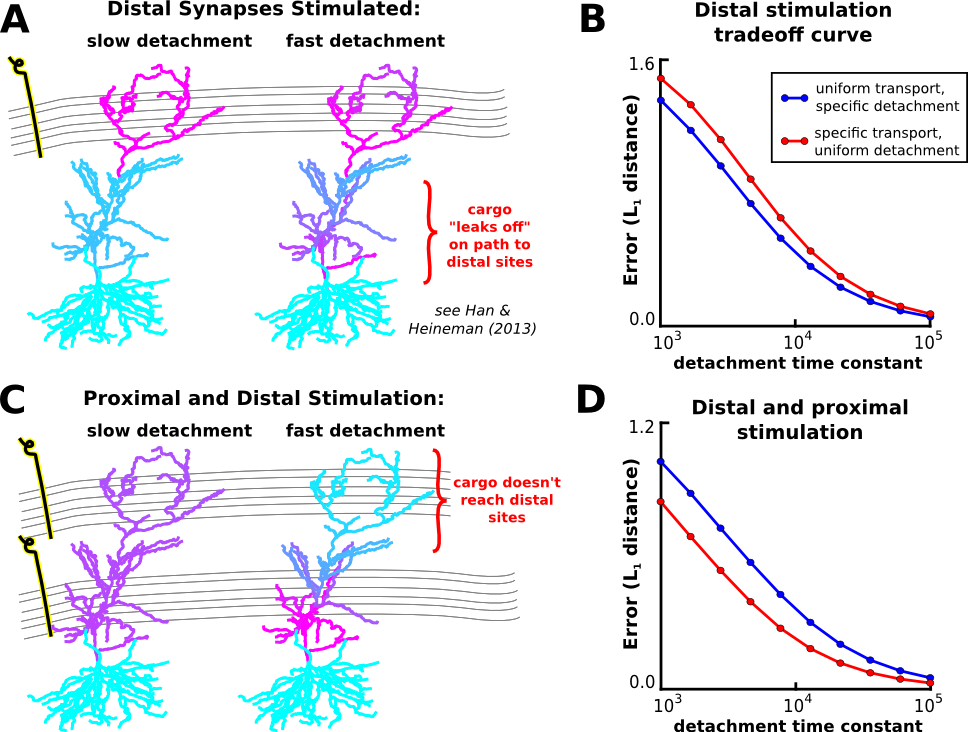
\includegraphics[width=0.9\columnwidth]{05_heterosynaptic_ca1.png}
\caption{Proximal synapses capture more cargo at the expense of distal synapses when detachment rates are n\"iavely increased.
\textbf{(A)} Delivery of cargo to the distal apical zone with slow \textit{(left)} and fast detachment rates \textit{(right)}. The steady-state cargo distribution does not match the stimulated pattern when detachment is fast. \textbf{(B)} Tradeoff curves between non-specificity and convergence rate for two trafficking strategies (blue line, see Fig 4D; red line, see Fig 4C). \textbf{(C-D)} Same as \textbf{(A-B)} but for cargo delivery to the entire apical tuft.
}
\end{center}
\end{figure}

To appreciate this, consider an experiment where distal synaptic inputs on the apical tuft are stimulated (Fig. 5A).
If the average detachment rate constants are sufficiently slow, then, as before, cargo is delivered selectively to the stimulated region (Fig. 5A, left).
If we increase the detachment rates by a uniformly scaling, some cargo ``leaks off'' the microtubule path on its way to the distal synapses (Fig. 5A, right).
We refer to this as a ``non-specific'' delivery of cargo, since cargo is not selectively delivered to the stimulated sites.
\hl{For this stimulation pattern, non-specificity might induce on-the-path synaptic plasticity; a possibility that has some experimental evidence} \citep{Han_2013}.

Tradeoff curves between the average detachment rate constant and the non-specificity of transport for this stimulation pattern are shown in figure 5B.
Importantly, this tradeoff exists for both trafficking strategies we examined in figure 4 --- the selective transport strategy (see Fig 4D) and uniform transport strategy (see Fig. 4C).
The uniform trafficking strategy (Fig. 5B, blue line) outperforms the specific trafficking strategy (Fig. 5B, red line) since the latter suffers from bottleneck in the proximal apical zone.

Different patterns of non-specificity occur for other stimulation patterns.
When the entire apical tree is stimulated, fast detachment can result in a complete occlusion of cargo delivery to distal synaptic sites (Fig. 5C).
As before, a tradeoff between specificity and delivery speed is present for both transport strategies (Fig. 5D).
Interestingly, the specific trafficking strategy outperforms the uniform trafficking strategy in this case (in contrast to Fig. 5A-B).
This is due to the lack of a bottleneck, and the fact that the uniform trafficking strategy initially sends cargo to the basal dendrites where it is not released.

\subsection*{Transport can be optimized for both speed and precision for a given stimulation pattern}

\hl{have detachment rate be tunable by amount of stuff present???}

In figure 5, we showed that scaling the detachment rates ($c_i$), while leaving the transport rates ($a_i$, $b_i$) fixed produces a proximal bias in cargo delivery.
That is, synapses closer to the soma are more likely to capture cargo at the expense of distal synapses.
We reasoned that increasing the anterograde transport rate of cargo could correct for this bias, producing transport rules that are both fast and precise.

We examined this possibility in a reduced model --- an unbranched cable --- so that we could develop simple heuristics that precisely achieve a desired distribution of cargo (more complex, \textit{ad hoc}, heuristics could be developed for complex morphologies).
In the reduced model, cargo begins on the left end of the cable and is transported to a number of synaptic sites, each of which is modeled as a double-exponential curve.

\begin{figure}[!tb]
\begin{center}
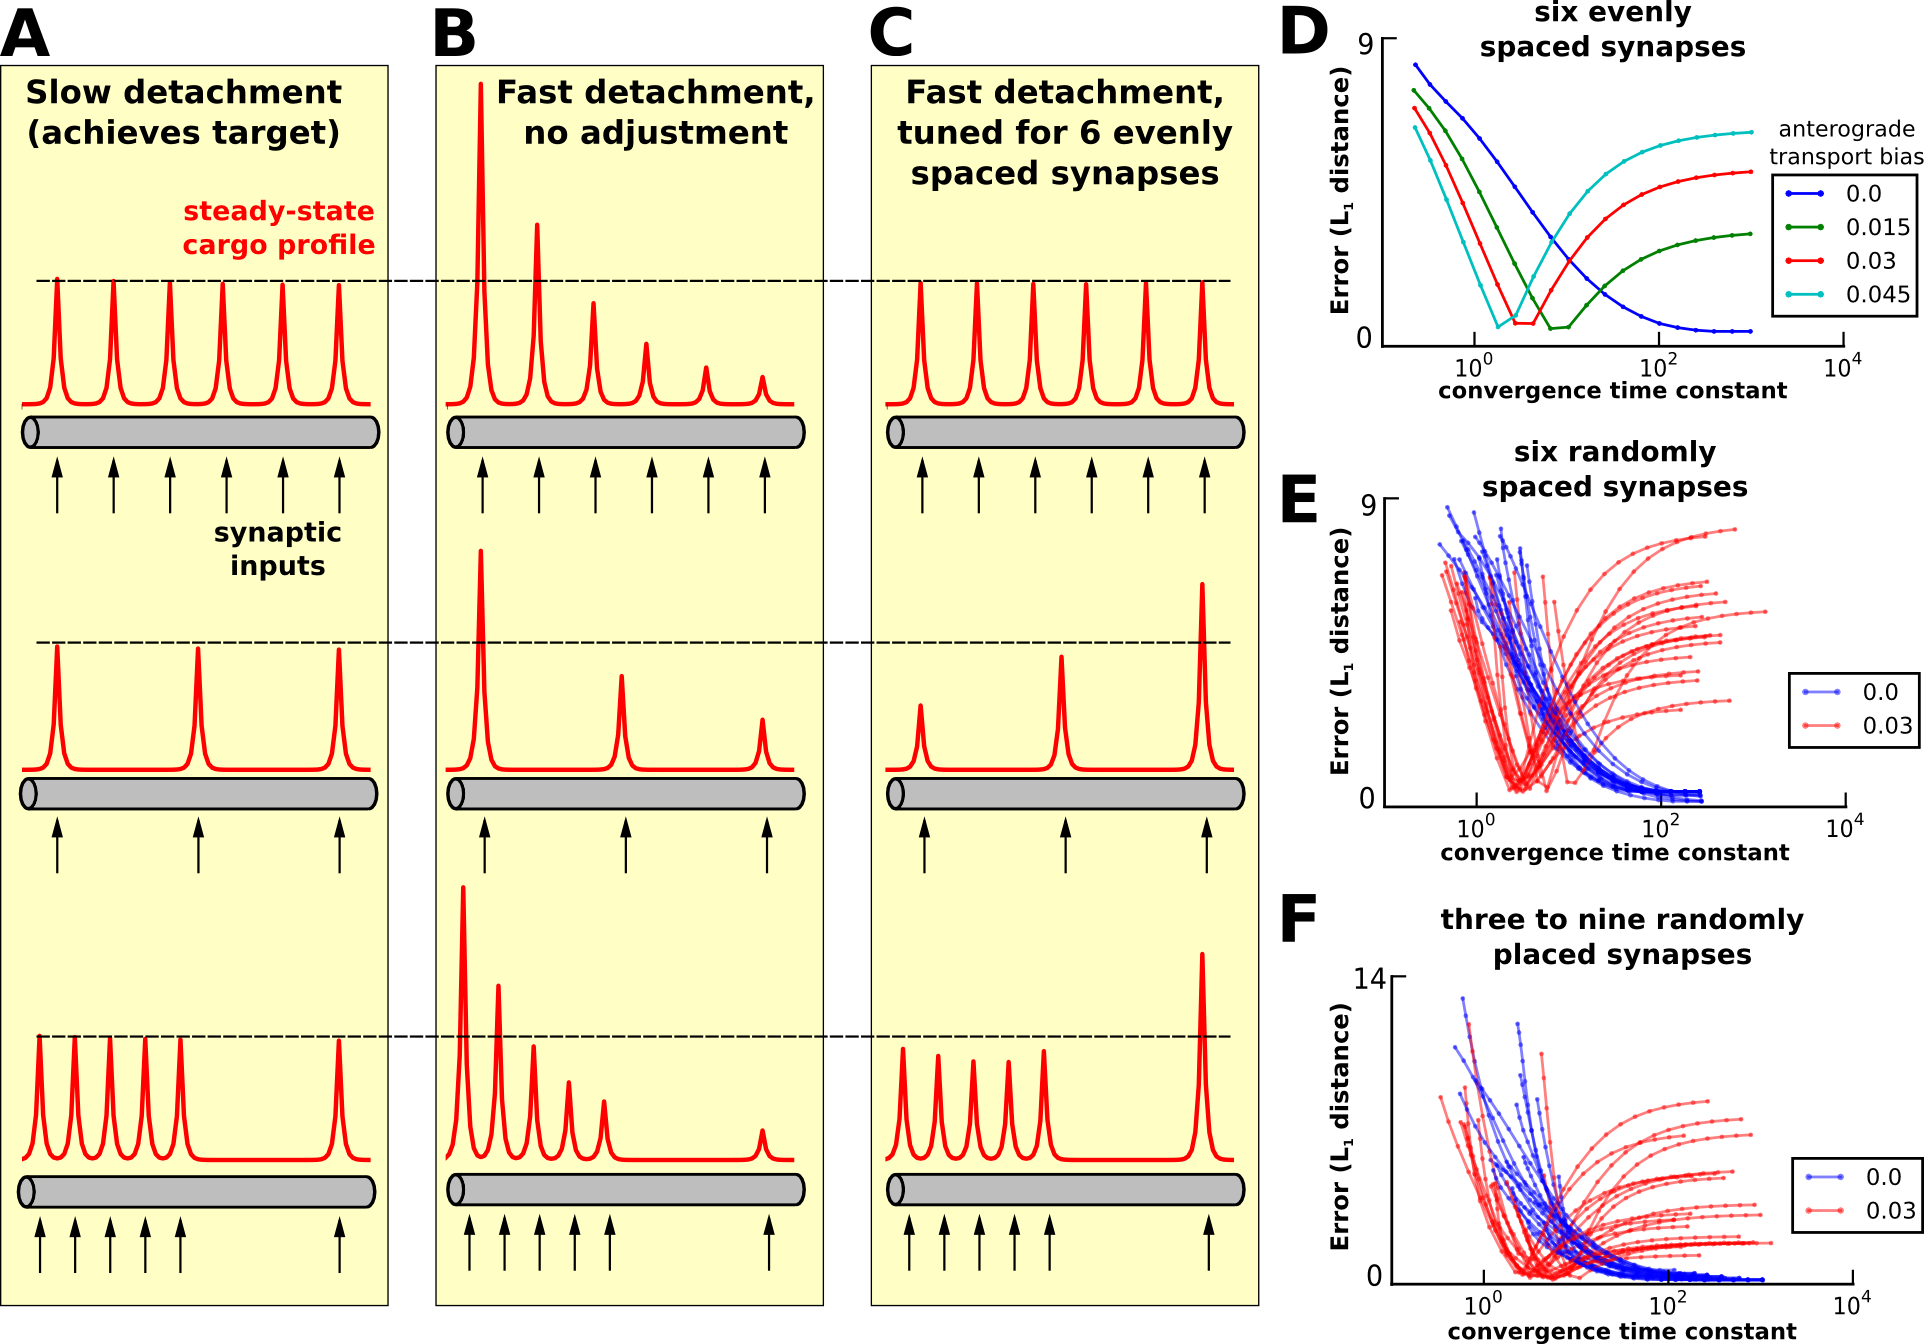
\includegraphics[width=0.9\columnwidth]{06_heterosynaptic_cable.png}
\caption{Producing speed and specificity for particular stimulation patterns does not extend to other patterns. Cargo begins on the left end and is transported to the right.
\textbf{(A-C)} Steady-state cargo profiles (red) for three stimulation patterns (black arrows) along an unbranched cable.
\textbf{(A)} When the timescale of detachment is sufficiently slow, cargo can be evenly distributed to the synapses regardless of their number and position. Transport parameters were set according to the procedure shown in figure 4D.
\textbf{(B)} When detachment is n\"iavely increased (all rates multiplicatively scaled) a proximal bias in the steady-state distribution of cargo across all stimulation patterns.
\textbf{(C)} Transport rate constants, $a_i$ and $b_i$, were tuned to optimize the distribution of cargo to six equally spaced synapses (top row); detachment rate constants were the same as in panel B. Changing the number of synapses (middle row) or the position of the synapses (bottom row) causes the unequal distribution of cargo to synapses.
}
\end{center}
\end{figure}

As before, cargo can be precisely delivered to a variety of stimulation patterns when the detachment rate is sufficiently slow (Fig. 6A); when the detachment rate is n\"iavely increased to speed up the rate of delivery, a proximal bias develops for all stimulation patterns (Fig. 6B).
This bias is qualitatively exponential.

We then hand-tuned the transport rate constants to deliver equal cargo to six evenly spaced synaptic sites (top row of Fig. 6C).
Specifically, we increased the anterograde rate constants ($a_i$) and decreased the retrograde rate constants ($b_i$) by a decreasing linear function of position so that $a_N = b_N$ at the right side of the cable (see Methods).
Intuitively, this pushes cargo past the proximal synaptic sites more quickly, canceling out the exponential delivery bias induced by fast detachment.

However, this tuned transport model does not precisely deliver cargo for other stimulation patterns.
When the number of synapses on the cable is decreased, a distal delivery bias is observed because too little cargo is released on the proximal portion of the cable (middle row, Fig. 6C).
Even when the number of synapses is held constant, changing the position of the synapses can disrupt equal distribution of cargo. This is shown in the bottom row of figure 6C, where a distal bias again develops when the majority of activated synapses are positioned proximally.
Thus, within the simple framework we've developed, the delivery of cargo can be tuned to achieve both precision and speed for a specified target distribution.
However, non-specific cargo delivery occurs when different stimulation patterns are applied (assuming the transport parameters are not re-tuned).

To examine these observations over a larger range of stimulation patterns and transport parameters, we plotted tradeoff curves between delivery precision and speed.
We first examined a cable with six evenly spaced delivery sites (same as top row of Fig. 6A-C).
As before, a hard tradeoff between specifity and delivery speed exists for the untuned model (blue line in Fig. 6D, same transport rate constants as Fig. 6A and 6B).
As the transport rate constants are tuned to increase anterograde movement, the optimal points along the tradeoff curve move to the left, representing faster transport times.
However, the tradeoff curves also become nonmonotonic: the error (non-specificity) initially decreases as the detachment rate decreases, but begins to increase after a certain well-matched point.
Points on the descending left branch of the curve represent cargo distributions with proximal bias (detachment is too fast); points on the ascending right branch correspond to distal bias (detachment is too slow).

We observed qualitatively similar tradeoff curves for randomly positioned synapses (Fig. 6E), and for randomizing the number and position of synapses (Fig. 6F). There is substantial variability in the tradeoff curves in both cases, but particularly when randomizing the number of synaptic inputs. Notably, the untuned transport model (blue curves) always converge to zero error as the detachment rate decreases. Thus, for this model, it appears that the only way to achieve very precise and flexible transport is to have a slow detachment rate.

\section*{Discussion}

A microscope image of a typical neuronal dendritic tree hints at the complex logistical task that the neuron must solve to maintain synapses and alter them, as appropriate, during development and learning.
Synapses, such as the extensively-studied excitatory synapses of the mammalian nervous system, comprise hundreds of different proteins, including receptors, structural and anchoring proteins, and cytosolic signalling enzymes [REFs].
How do these components find their way to the synapse, and how do synapses that have varying demands for these components receive an appropriate supply?

Local protein synthesis near synaptic sites offers an elegant solution to this problem.
Many mRNAs for synaptic proteins are distributed in dendrites, along with ribosomes and translational regulation machinery that can provide new proteins as they are needed [REFs].
However, these components need to be appropriately distributed to begin with and on a long timescale their distribution needs to be maintained.
On the other hand, some forms of long-term synaptic plasticity have a transcription-dependent component, suggesting that somatic biosynthesis and dendritic trafficking are important for maintaining and controlling synaptic connectivity in addition to local mechanisms.

We examined simple models of microtubular transport to investigate how such a global network can be organized and controlled in complex neuronal morphologies.
Previous models of microtubular-based transport have examined systems with spatially uniform rates of anterograde and retrograde transport \citep{Smith_2001,Bressloff_2006}.
We hypothesized that complex spatial patterns could emerge by relaxing this assumption. One might na\"ively expect that elaborately branched morphologies obfuscate the relationship between these local mechanisms and the global distribution of molecular cargo.
We showed that the relationship is actually quite simple: the steady-state ratio between neighboring compartments is the reciprocal ratio of the trafficking rate constants connecting those compartments.

Local activity signals provide a means to sequester dendritic cargo as it passes a synapse, providing a way for plasticity-inducing synaptic stimulation to `tag' a synapse.
Direct evidence of activity-dependent arrest \citep{Soundararajan_2014} and accumulation \citep{Krichevsky_2001,Buxbaum_2014a} of mRNAs and other actively transported biomolecules suggests that the kind of mechanism we studied here is involved in regulating synapses in parallel with local synthesis mechanisms.
We are agnostic about the precise identity of the activity signal that controls transport and sequestration, but note that experiments have shown that local calcium \citep{Wang_2009} and ADP \citep{Mironov_2007}, alter anterograde and retrograde transport rates.
Similarly, experimental data indicate that degradation of mRNA can be spatially heterogeneous and activity-dependent \citep{Farris_2014}.
Incorporating these additional processes into the model created new possibilities for molecular trafficking; the same expression pattern can be achieved by nonuniform microtubular transport followed by uniform release or from uniform transport followed by nonuniform release (Fig. 4).

There is experimental evidence for both strategies. \cite{Kim_2015} identified three mRNAs that were uniformly distributed throughout cultured \textit{Aplysia} sensory neurons, but were targeted to synapses at the level of protein expression by localized translation.
In contrast, the nonuniform expression of \textit{Arc} mRNA is closely matched to the pattern of Arc protein \citep{Farris_2014, Steward_2015}. 

Each of these transport strategies might be tailored for different constraints or purposes.
For example, a uniform mRNA profile could facilitate shifts in the protein expression pattern, since the changing the pattern of local translation is presumably faster than re-distributing the mRNA.
In other cases, it might be undesirable to rapidly shift protein expression based on transient changes to the neuron or circuit; controlling expression at the level of mRNA might prevent this.
We showed that it is possible to interpolate between these two strategies (Fig. 4E), which might allow neurons to trade off between the relative advantages of each.

FRX - in this disease there is aberrantly high translation of mRNAs. This is like a high sequestration rate. Leads to higher connectivity but perhaps lower specificity.

Other assumptions of the mass-action model - Second, the model assumes are many copies of $u$ in each compartment.This allows us to approximate the mass as a continuous variable, and the dynamics of the system as deterministic.Third, the number of molecular motors and capacity of the microtubules is not saturated by the level of $u$ in any compartment. This means that the rate of transport from compartment A to compartment B linearly increases with the amount of $u$ in compartment A.

\section*{Methods}

\subsection*{Microtubule Transport Model (Fig. 1)}
Transport in an unbranched cable (equation 1) leads to the following system of differential equations:
$$
\begin{array}{lcl}
\dot{u}_1 & = & -a_1 u_1 + b_1 u_2 \\
\dot{u}_2 & = & a_1 u_1 - (a_2+b_1) u_2 + b_2 u_3 \\
~ & \vdots & ~ \\
\dot{u}_i & = & a_{i-1} u_{i-1} - (a_i+b_{i-1}) u_i + b_i u_{i+1} \\
~ & \vdots & ~ \\
\dot{u}_N & = & a_{N-1} u_{N-1} - b_{N-1} u_N 
\end{array}
$$
Similar systems result from branched mass-action models. The steady-state relationship in equation 5 can be immediately verified at either end of the cable:
$$
\dot{u}_1 = 0 ~\Rightarrow~ -a_{1} u_{1} + b_{1} u_2 = 0 ~\Rightarrow~ \frac{u_1}{u_2} \Bigg |_{ss} = \frac{b_1}{a_1}
$$
The same procedure can be iteratively applied down the cable to show that equation 5 holds globally. The same result can be shown in a branched tree morphology. Here, each compartment has exactly one parent, but can have multiple children at branch points. Consider a parent-child pair of compartments, $u_p$ and $u_c$, with anterograde/retrograde transport rate constants $a$ and $b$. At steady-state, there is no net flux between $u_c$ and its children:
$$
\dot{u}_c = a u_p - b u_c + \underbrace{\sum_j (b_j u_j - a_j u_c)}_{= 0 \text{ , at ss}}
$$
Thus, we have:
$$
\dot{u}_c = a u_p - b u_c = 0 ~\Rightarrow~ \frac{u_p}{u_c} \Bigg |_{ss} = \frac{b}{a}
$$
To study how the system converges to steady-state, we can re-express the model as a matrix differential equation, $\mathbf{\dot{u}} = A \mathbf{u}$, where $\mathbf{u} = \left[ u_1, u_2, ... u_N \right]^T$ is the state vector, and $A$ is a matrix. For a general branched morphology, the matrix $A$ will be nearly tridiagonal, with off-diagonal elements corresponding to branch points; matrices in this form are called Hines matrices \citep{Hines_1984}. For the simpler case of an unbranched cable, $A$ is tridiagonal:
$$
A = 
 \begin{bmatrix}
  ~-a_1~  & b_1      & 0         &         & ...              & 0        \\
   a_1    & -b_1-a_2 & b_2       &  0      &                  &          \\
   0      &  a_2     & -b_2-a_3  & ~~~ b_3~~~  & \ddots     & \vdots   \\
   \vdots &  0       & a_3       & \ddots  &                  & 0        \\
          &          & \ddots    &         & -b_{N-2}-a_{N-1} & b_{N-1}  \\
   0      &          & ...       &  0      & a_{N-1}          & ~-b_{N-1}~
 \end{bmatrix}
$$
For both branched and unbranched morphologies, each column of $A$ sums to zero, which reflects conservation of mass within the system. The rank of $A$ is exactly $N-1$ (this can be seen by taking the sum of the first $N-1$ rows, which results in $-1$ times the final row). Thus, the nullspace of $A$ is one-dimensional (red lines in Supp. Fig. 1).

The desired distribution, $\mathbf{\tilde{u}}$, is an eigenvector that spans the nullspace of $A$. All other eigenvalues $A$ are negative, which can be shown using the Gershgorin circle theorem. The convergence rate is determined by the non-zero eigenvalue with smallest magnitude of $A$. We can increase the convergence rate (while still maintaining $\mathbf{\tilde{u}}$) by multiplying all rate constants by some common value. However, this trivial strategy ignores the fact that there are biophysical limits on how fast molecular motors can move.

\subsection*{Stochastic Model of Transport}

We model the stochastic transport of a single molecule with a discrete-time Markov chain model. Let the vector $\mathbf{p}^{(k)} = [p_1^{(k)}, p_2^{(k)}, ..., p_N^{(k)}]^T$ denote the probability of finding the molecule in each of the $N$ compartments on the $k$th time step. For example, $p_1^{(0)}$ is the initial probability that the molecule is in the first compartment (which is the soma in our implementation). The state-transition matrix $S$ describes the probabilistic anterograde/retrograde transport of the molecule between neighboring compartments in each discrete time step:
$$
\mathbf{p}^{(k+1)} = S\mathbf{p}^{(k)}
$$
The state-transition matrix is related to the mass-action system matrix $A$ by the following relation:
$$
S = \Delta t A + I
$$
where $\Delta t$ is the length of a time step (assumed to be very small), and $I$ is the identity matrix. The columns of $S$ sum to one, and, since $\Delta t$ is small, all elements of $S$ lie on the interval $[0,1]$. This transformation shifts and scales the eigenvalues of $A$ to lie on the interval $(0,1]$, without modifying the eigenvectors of the system. The steady-state probability distribution is given by the eigenvector of $S$ with eigenvalue 1 (CITE), which is identical to the vector spanning the nullspace of $A$ and therefore the steady-state concentration distribution of the mass-action model.

\subsection{Transport Model With Detachment and Degradation (Fig. 4)}

We can also interpolate between these two strategies to achieve the target distribution. Let $F$ be a scalar between 0 and 1, and let $\tilde{u}^\star$ be normalized to sum to one. We choose $a_i$ and $b_i$ to achieve:
$$
\tilde{u}_i = F~\tilde{u}_i^\star + (1-F)/N 
$$
along the microtubular network and choose $c_i$ to satisfy
$$
c_i \propto \frac{\tilde{u}_i^\star}{F~\tilde{u}_i^\star + (1-F)/N} 
$$
Here, $N$ is the number of compartments in the model. Setting $F=1$ results in the simulation in figure 4C, while setting $F=0$ results in the simulation in figure 4D. Setting $F=0.3$ results in the simulation shown in figure 4E, which uses an interpolated strategy.


\section*{Acknowledgements}

\bibliography{transport_refs}

\end{document}